%---------------------------------------------------------------------------------------------------
% Modellierung
%---------------------------------------------------------------------------------------------------
\section{Modellierung}

Das Experiment besteht grob aus drei Phasen:
\begin{itemize}
  \item Aufstieg im Ballon
  \item Absprung und freier Fall
  \item Gebremster Fall am Fallschirm und Landung
\end{itemize}
Der Aufstieg wird im Rahmen dieser Arbeit nicht weiter betrachtet.
Interessanter ist der Fall - vor allem der ungebremste Abschnitt von Absprung bis zum Öffnen des Fallschirms.
Um dies zu simulieren, müssen relevante Kräfte und Größen berücksichtigt werden. %identifiziert und modelliert werden.

Auf den Springer und seine Ausrüstung wirken lediglich zwei Kräfte:
\begin{description}
  \item[$F_g$] Zur Erde hin wirkt die Gravitation.
  \item[$F_L$] Bremsend wirkt der Luftwiderstand, der sich bei Öffnen des Fallschirms massiv erhöht.
\end{description}

Die ausschlaggebenden Größen werden im Folgenden beschrieben.


\subsection{Gravitation}
Die Gravitation wirkt zwischen dem Springer und der Erde.
Allgemein wird hier das newtonsches Gravitationsgesetz angewendet.
\begin{equation}
F_g=G \frac{m_1 m_2}{r^2}
\end{equation}
Dabei ist $G$ die Gravitationskonstante $6.67384\times 10^{-11} \frac{m^3}{kg\ s^2}$, $m_1$ und $m_2$ die beteiligten Massen und $r$ deren Abstand.

Bis auf $r$ (der Springer bewegt sich ja auf die Erde zu) sind hier alle Größen konstant.
$r$ ist dabei gleich dem Radius der Erde plus der Höhe des Springers \vgl Abb.~\ref{fig:gravitation}.
\begin{figure}[h]
  \centering
  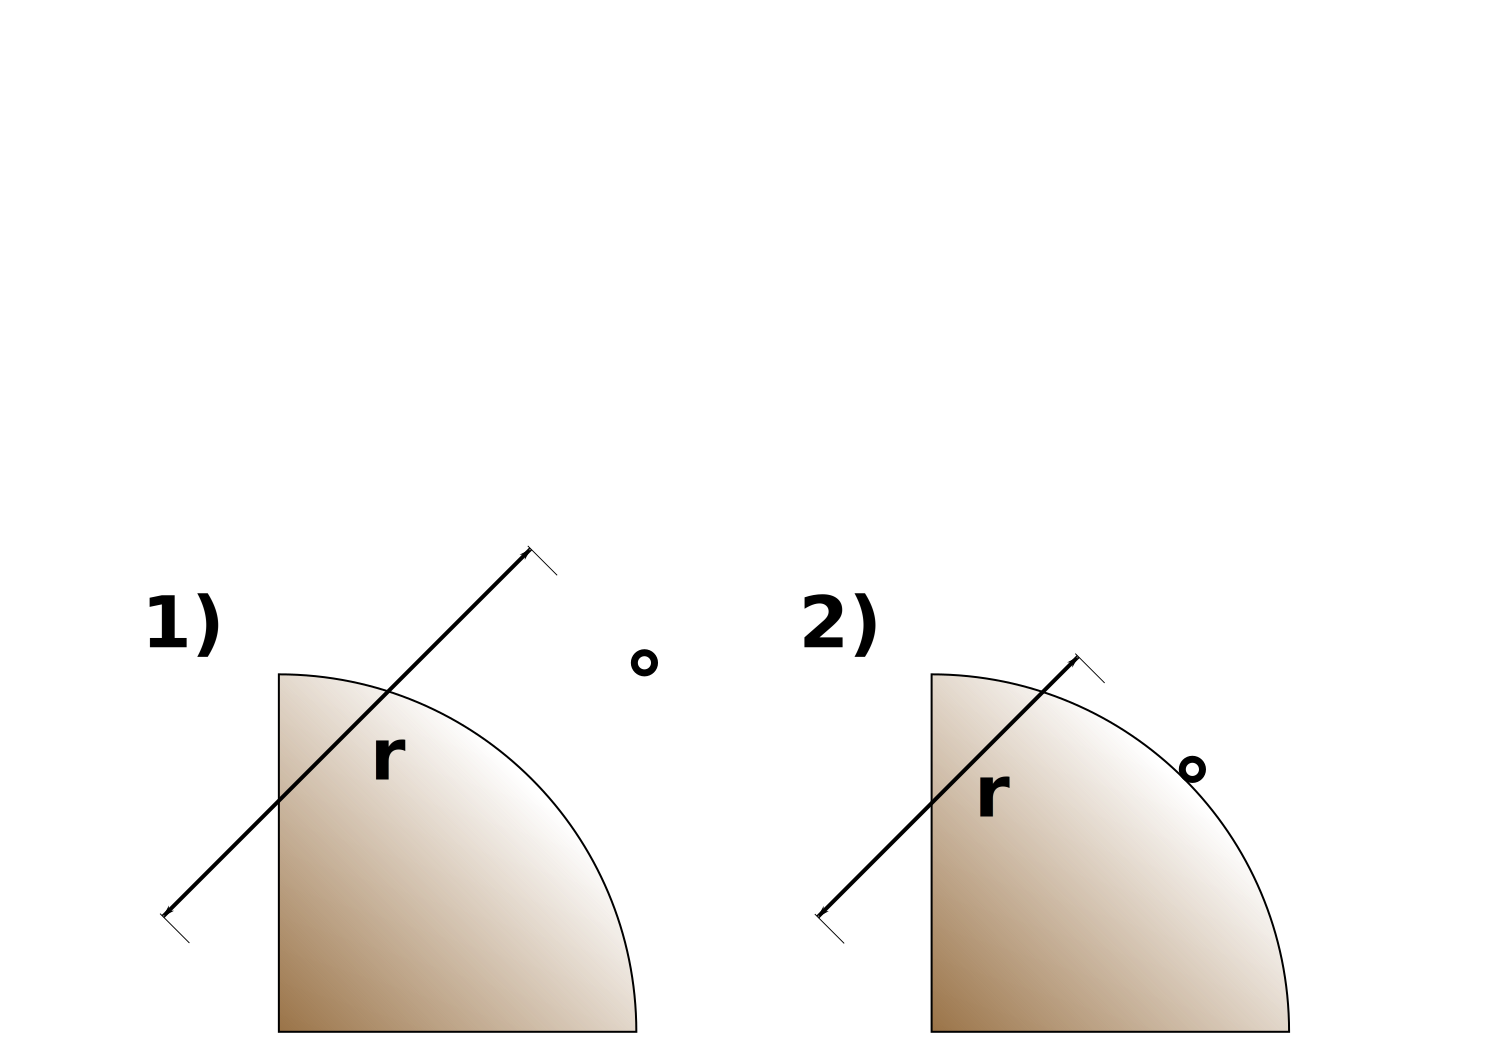
\includegraphics[width=0.5\textwidth]{gravitation}
  \caption{$r$ bei 1) Absprung und 2) Landung}
  \label{fig:gravitation}
\end{figure}


\subsection{Atmosphäre}
Die Atmosphäre ist keine homogene Gasblase.
Sie ist komplexer aufgebaut.
Für die Simulation sind dabei die Temperatur und die Dichte in der jeweiligen Höhe von Bedeutung.

\subsubsection{Dichte}
Mit steigender Höhe nimmt die Dichte ab, da die darüberliegendes Gassäule kürzer wird.


\subsubsection{Temperatur}



\subsection{Strömungswiderstand}

\subsubsection{Überschallflug}



